\graphicspath{{"./Chapter 2/Karsts/"}}

\chapter{Generation of karst networks}
\label{chap:karsts}

\teaser {
    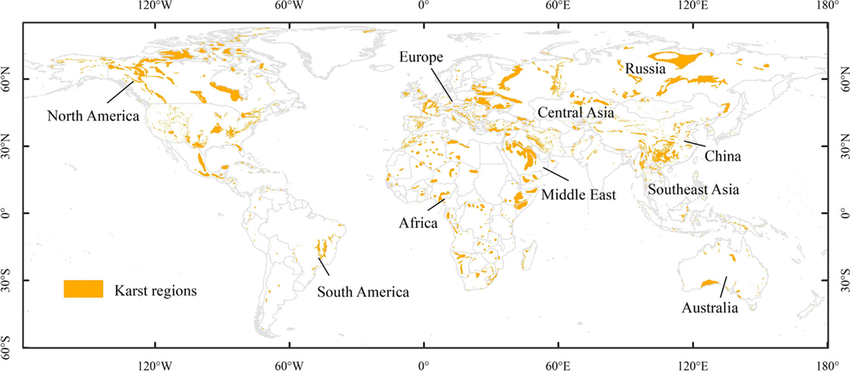
\includegraphics{Global-distribution-of-karst-regions.png}
    \caption{Karst networks can be find anywhere on Earth. Source: \citep{Huang2022}.}
    \label{fig:karsts_distribution}
}

\abstract
During this thesis, a novel method for the generation of karst networks have been proposed. This method is tailored by the idea of proposing fast and highly controlable methods to create geologic features. We used an adaptation of a procedural vegetation generation algorithm with very few additions. As this work does not propose an innovation but instead presents a possibility to cross the works from different research domains, we added this chapter as an appendix, such that other computer graphics works might be inspired by it.


\minitoc

\section{Introduction}
\label{sec:karst_introduction}
Karst networks are complex subterranean systems formed primarily in soluble rocks like limestone, dolomite, and gypsum. Their formation takes thousands to millions of years. Over time, groundwater erodes the rock, creating intricate, often interconnected systems of caves and conduits. We can find these formations all over the world (\cref{fig:karsts_distribution}).

Karst networks offer unique ecosystems, as they are isolated from the exterior biotic and abiotic factors such as light, oxygen, etc... They contain at the same time terrestrial and underwater environments, then populated by trauglofauna and stygofauna (respectively terrestrial and aquatic animals living in complete darkness). This environment maintain stable temperatures and high humidity, providing a consistent microclimate during all seasons. This can support a range of life forms, from microbes to small vertebrates, that survive in low-energy environments.

A karst network forms through a process called chemical weathering, more specifically carbonation, where soluble rocks like limestone, dolomite, and gypsum are dissolved by slightly acidic water over long periods of time.  Rainwater absorbs carbon dioxide (\ch{CO2}) from the atmosphere and from organic material in the soil, forming a weak solution of carbonic acid (\ch{H2CO3}). Water infiltrates through joints, fractures, and bedding planes (the natural layers in the rock). Initially, these cracks are small, but as water continuously dissolves the rock along these lines of weakness, the cracks enlarge, creating conduits for water to flow more easily. Water percolates through cracks in the bedrock, it reacts with calcium carbonate in limestone, dissolving the rock in a chemical reaction. This reaction results in calcium ions (\ch{Ca^{2+}}) and bicarbonate ions (\ch{HCO3^{-}}) being carried away by groundwater, slowly enlarging the cracks and fractures in the rock. As the water continues to dissolve rock along these pathways, small cracks can grow into large underground channels or tunnels, which are the beginnings of cave systems. Over time, these underground channels expand into larger voids, forming caves.

Many factors influence the speed and size of karst formations. The main factors are:
\begin{Itemize}
    \Item{} The rock composition, which can have different concentration [CHECK THIS TERM] of \ch{CaCO3}, reacting more or less with acidic water and thus resisting proportionnaly to the erosion.
    \Item{} Fractured bedrock facilitate the water pathway, easing the weathering process in a certain direction. 
    \Item{} Surface vegetation density also plays an important role as it produces \ch{CO2} that is being drained by rain water, accelerating the carbonation of the bedrock. Precipitation and atmospheric humidity increase the amount of infiltrated water. These environment parameters are significantly correlated \cite{Bari2021}.
\end{Itemize}

Karst systems have an important role in the environment as they enable the storage and purification of ground water while providing a continuous water flow at the surface. This feature have a large impact for the surface environment, as it serves as aquifer and drought buffer, which is useful for the surface ecosystems or human agriculture.

Karst subterrains can be seen as networks of caves connected through channels with sizes that varies greatly \cite{Collon2017,Collon2021}. The underground study is a difficult task as the channels can become too small for a human, and can be fully submerged for an undefined distance, making spelaeological expeditions dangerous. Important technologies have arise such as LIDAR for the 3D modeling of explored caves and underground-GPS systems for studying the system's topology \cite{Collon2017}.



% - Importance: significant for water resources, unique ecosystems, and land use management. \\
% - Formation and development \\
% ** Chemical weathering \\
% *** Study the role of rainwater acidity (carbonic acid) in dissolving carbonate minerals. \\
% ** Underground drainage \\
% *** Analyze the development of subterranean drainage systems, including caves, tunnels, and sinkholes. \\
% ** Speleogenesis \\
% *** Examine the process of cave formation, especially at or below the water table. \\
% - Key features of karst networks \\
% ** Caves and caverns \\
% *** Document major cave systems and their formation processes. \\
% ** Sinkholes (dolines) \\
% *** Identify areas prone to sinkhole formation and study their causes. \\
% ** Disappearing streams and springs \\
% *** Trace the path of streams that vanish into the ground and re-emerge. \\
% ** Karst valleys \\
% *** Investigate valleys formed by the collapse of underground voids. \\
% ** Stalactites and stalagmites \\
% *** Study the formation of these features within caves. \\
% - Hydrology of karst networks \\
% ** Aquifers \\
% *** Assess the productivity and structure of karst aquifers. \\
% ** Groundwater flow \\
% *** Model the rapid and turbulent flow of water through karst systems. \\
% ** Vulnerability to contamination \\
% *** Evaluate the risks and sources of contamination in karst aquifers. \\
% - Ecology of karst environments \\
% ** Unique habitats \\
% *** Research cave-dwelling species (troglobites) and their adaptations. \\
% ** Biodiversity hotspots \\
% *** Identify and document biodiversity hotspots in karst regions. \\
% - Human interaction with karst networks \\
% ** Water resources \\
% *** Study the dependence of regions on karst aquifers for freshwater. \\
% ** Tourism \\
% *** Assess the impact of tourism on karst landscapes and caves. \\
% ** Land use challenges \\
% *** Develop guidelines for construction and land use planning in karst regions. \\
% ** Environmental concerns \\
% *** Identify and mitigate pollution and land degradation impacts. \\
% - Examples of karst regions \\
% ** The Mammoth Cave System (USA): world's longest cave system. \\
% ** The Guilin Karst (China): unique limestone peaks and river systems. \\
% ** The Dinaric Karst (Balkans): extensive cave systems and karst phenomena. \\
% - Research and study in karst science \\
% ** Speleology \\
% *** Promote the scientific study of caves and karst features. \\
% ** Geohydrology \\
% *** Conduct studies on water flow in karst systems for resource management. \\
% ** Geomorphology \\
% *** Research the development of karst landforms over geological timescales. \\


\section{Related works}
\label{sec:karsts_related-works}
- Modeling based on geology (no control): \\
** \cite{Jaquet2004,Pardo2012}
- State of the art: \\
** \cite{Paris2021}, more recently \cite{Gouy2024} \\
*** In our case, we do not rely on a graph and path finder, which allows us to compute sections of the karst on the fly (no need to know the whole network to find paths) \\
*** Plus, the computation of sampling and cost graphs can be very expensive, reducing possibilities of user interaction. 
*** Fractures typically form due to changes in overlying pressure or tectonic stress from faulting or folding. To gain a more comprehensive understanding of the location, orientation, and extent of fractures in rock, as well as their hydrogeologic behavior, geophysical surveys can be useful. These investigations can employ a variety of geophysical tools, including surface geophysical instruments (non-invasive) and downhole geophysical logging, which requires a borehole. However, numerical simulation of bedrock fractures is highly complex and demands a deep understanding of the surrounding environment to achieve accurate results. \\
** \cite{Pytel2015} \\
*** Based on voxels, looks plausible, with a low number of parameters, but take way too long (\~10 to 20 minutes per generation) \\
*** Which makes it unfit for user interaction \\
** \cite{Collon2015,Collon2017,Jouves2017} \\
- With some imagination, we can see the shape of trees: \\
** [Prusinkiewicz : ANY] \\
** \cite{Runions2008} \\
- Or miscelleanous networks: \\
** \cite{Galin2010, DiasFernandes2018} \\
- Maybe even look for lychen or ant colonies \\
- ...

\section{Space colonization}
\label{sec:karsts_space-colonization}
- Not really a tree, but... \\
** Some networks are branching \\
** Some have low number of cycles \\
- SC is easy to manipulate for an user \\
- For these reasons, we will consider the use of SC. \\
- Description of the algorithm: \\
** Definition of a root and sinks \\
** Evolution from the root toward closest sinks \\
** Branching [WHEN NEEDED] \\
- ...

\section{Our method}
\label{sec:karsts_our-method}
- Based on classic SC \\
** Merging branches \\
** Closing paths based on angle and distances to create cycles \\
- Adding width to the branches \\
** Destroying paths when width too small \\
- Leaves as chambers/cavities \\
- ... 

\section{Modeling}
\label{sec:karsts_modeling}
- Tunnels: \\
** The output of SC is a set of paths \\
** \cite{Paris2021} provides a classification of tunnel shapes (\cref{fig:karsts_tunnel-classif}). \\
- ...

\begin{figure}
    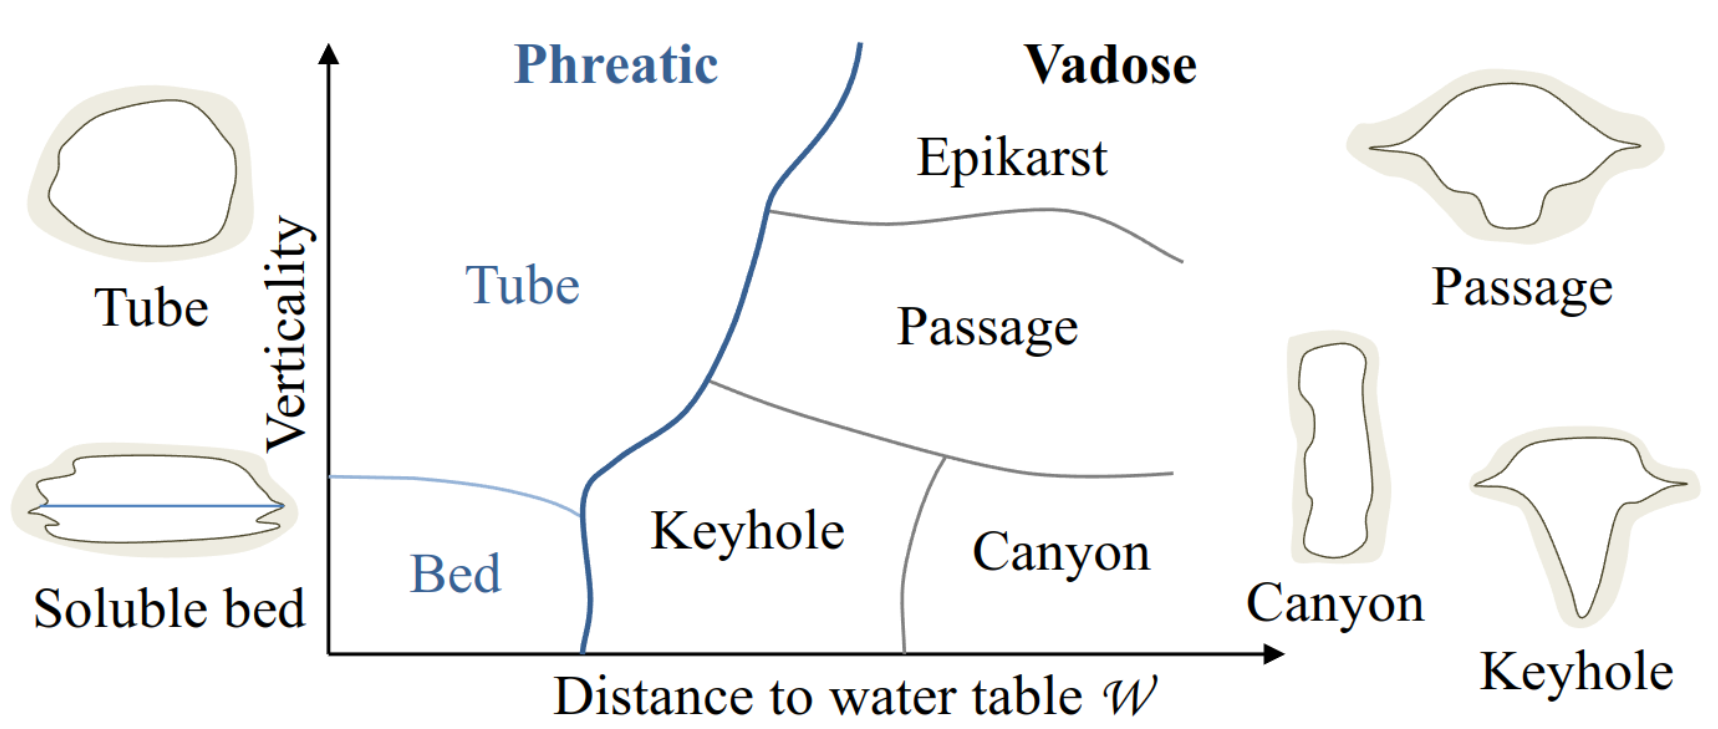
\includegraphics{KarstClassificationParis}
    \caption{Classification of tunnel shapes}
    \label{fig:karsts_tunnel-classif}
\end{figure}

\section{User control}
\label{sec:karsts_user-control}
- Importance of keeping user control \\
** Shape of a karst is close to randomness \\
** Want to be predictible \\
- Manipulation of control points \\
** Source \\
** Sink \\
- Paths tortuosity \\
- Inclusion of soil properties in the formation of paths, using the gradient of: \\
** Humidity, \\
** Porosity \\
- Real-time editing \\
** Allows for precise manipulation \\
- ...

\section{Results}
\label{sec:karsts_results}
- ... 

\section{Conclusion}
\label{sec:karsts_conclusion}
- ...